\chapter{Conclusion: Where Next for Molecular Studies of CFTR}
\label{chap:conclusion}
\begin{chapquote} {Eduardo Perozo (personal communication)}
We have more problems than hands. 
\end{chapquote}


\section{Summary: The Three Important Categories for Future CFTR Studies}

As figure \ref{CF_life_expectancy} demonstrated back in chapter \ref{chap:cftr}, basic science discoveries concerning CF have had a direct effect on the lives of patients. The work in this thesis is a small example of this. We have applied the abstract physical models outlined in \ref{chap:methods} understand genetic mutations carried by real patients. It is hoped that our findings can help to collect evidence which will give more patients access to medications which could add decades to their lives span. In this final chapter we will outline a set of \textit{in silico} studies which will allow a more mechanistic approach to the theratyping of CFTR mutations, and hopefully give more patients access to the medications which are right for them.  

The studies we will propose are now possible because we are entering an exciting era of biophysical research---where advances in theoretical methods, computing power and experimental techniques are beginning to drive each other at a frenetic pace. An example can be seen in the development of something like Alphafold2 \cite{jumper2021}. The maturation of cryo-EM allowed the discovery of new protein folds, which Alphafold2's machine learning algorithms could then learn from. With this data in hand, the algorithms could predict the structure of entire proteomes. Now, this means that structural biologists can use the predictions of Alphafold to solve even more structures more quickly. 

In the case of our work, as we collect more \textit{in vitro} biophysical data about CFTR, and perform more \textit{in silico} studies, we can refine the model in \ref{chap:perspective} further. Eventually, this would mean a portion of the experimental work currently performed by our collaborators will not need to be done, as their outcomes could be predicted with computers. This can also free up the experimental resources, to pursue other projects which are out of reach for computational models. 

In pursuit of this goal, below we have identified the three areas which will extend the computational reach of the model we have sought to build in this thesis, so it can make more useful prediction. This philosophy could one day be used to make a more patient specific choice for CFTR modulators, by further refining our molecular understanding of CF pathogenesis.

\begin{itemize}
	\item A basic understanding of the function of CFTR.
	\item Granular classification of CF-causing mutations and the biophysical basis for their misfunction.
	\item Elucidating the molecular mechanism of action of different CFTR modulators. 
\end{itemize}

In the next few sections we will suggest \textit{in silico} studies to further research in each of these areas. Each piece of this program can be related to the physical model we proposed in the last chapter. However, the most pressing area of research is not listed above---as it is completely beyond our computational capabilities at present. In order to make a more informed choice of modulators for each patient, the basis of the heterogeneous response amongst patients with the same genotypes must be understood \cite{hanafin2021}. 

Identification of which genetic and cellular factors give rise to this phenomenon will be critical to the development of personal medicine in CF. Without understanding the reasons behind this phenomenon, the mechanistic understanding we propose here will be obscured behind biological noise. Thankfully, it seems as though the personalised approach employed by our experimental collaborators is well placed to take on this task.

\section{Outstanding Basic Questions of CFTR Function}

Please take this opportunity to again inspect the proposed model in the last chapter again (Figure \ref{drug_action_model}). Note how the effects of mutations and drugs are both made relative to the underlying energy landscape of WT-CFTR. Hence, the first point in our proposed program, to understand the basic functions of CFTR, forms the basis of the model and should be given priority.

%Throughout this work we ahve found that disease causing mutation often have a unique mode of misfunction. What have found is a large diversity of molecular phenotypes which may cause disease. What is thus remarkable is that the \textit{in vitro} component of these papers all demonstrate that these mutations are responding to the same drugs, albeit with differing efficacies.

Perhaps the most important and also the most difficult study that needs to be performed is the simulation of CFTR's full gating cycle, to calculate the energetics in each step of the process. This will aid in the generation of new potentiators, but also serve as an important mile-stone in computational biophysics.

Since CFTR has been studied intensely, we know the energetics and the kinetics of its gating cycle very well \cite{csanady2017}. Matching existing experimental values would demonstrate the power of modern forcefields and free energy techniques. Recent simulations of the Covid spike protein have demonstrated this is likely now possible \cite{casalino2021}. Cryo-EM structures of ABC transporters in transient states could also be used to choose CVs and seed a SMwST or an eBDims based calculation \cite{hofmann2019, orellana2016, roux2021, pan2008}. 

With the help of our \textit{untargetted} simulations in chapter \ref{chap:opening}, we now have both the open and closed states of the CFTR---meaning a \textit{targeted} MD methodology could link them together \cite{zhang2018, liu2017}. A similar study was completed in 2015 on a small antiporter and with new computational engines the same is likely now possible for CFTR as well\cite{moradi2015}.

Characterising the energetics of the full gating cycle would form the basis of a quantitative version of the model proposed in chapter \ref{chap:perspective}.

\section{Mechanistic Understanding of Mutations}
As outlined in Figure \ref{granular_classification}, the molecular fingerprint of a CF causing mutation can be quite complex. Further work is needed to meaningfully group mutations into more categories which will help predict their response to modulators. We predict that the conventional 6 classes of misfunction will be split up over time, as has already begun in the literature \cite{veit2016}. 

By understanding the molecular defect of each mutation, we can think about how each one can be treated with specific modulators. Hence, once the gating cycle study suggested in the previous section is complete for WT-CFTR, the same protocol should also be applied to gating class mutants as well. This will help us understand \textit{where} in the energy landscape of the gating cycle a mutation causes a perturbation. Once the deleterious area is identified, it will give a rational basis for the grouping of theratypes, as we did with Q1291H in the last chapter.

In the absence of calculations of the full gating cycle, similar studies to this thesis could be carried out to identify different theratypes. This would involve systematically working through different mutations in each domain and drawing connections between them to identify networks of allostery. This could be completed with the help of Dynamics Network Analysis (DNA) \cite{melo2020}. 

From the perspective of protein physics, we should be optimistic about molecular theratyping of rare CFTR mutants. Given that $\Delta$F508 may be rescued by a triple therapy, we can expect that the vast majority of missense mutations are also amenable to pharmacological rescue. This is because the $\Delta$F508 mutation in fact represents a far more deleterious effect on CFTR the protein than many missense mutations \cite{bahia2021}. Hence, from our biophysical point of view, it makes little sense to exclude patients carrying the majority of these missense mutations from access to modulator therapy. The rationale for such exclusion is based upon the extreme cost of the drugs, alongside the unpredictability of patient response. 

However, it is unlikely that the reason patients with these rare missense mutations do not respond to modulators is due to the failure of modulators to act mutant forms of CFTR. Rather, when a patient does not respond to modulator therapy it is more likely due to poorly understood molecular or cellular factors we mentioned earlier. Given the findings of this thesis and the current understanding of the literature, we encourage a more rational, patient specific approach to the inclusion missense mutations in access to CFTR modulators. 


\section{Elucidating Modulator Action on CFTR}

The final area of our proposed programme concerns the molecular mechanism behind how modulators are acting on CFTR to restore its function. \textit{In vitro} protocols have recently been developed to test \textit{where} on the CFTR protein drugs bind, which will likely be very useful for future drug development \cite{laselva2022}. However, these efforts would be greatly aided by \textit{in silico} studies. It is currently unclear what these drugs are doing, at the molecular level, to deliver their therapeutic benefit. By elucidating this mechanism, we can design more potent modulators and give all patients more options. 

At the time of writing there are several studies which purport to have found binding sites for potentiators class drugs \cite{yeh2019, laselva2021a, liu2019, baatallah2021}. The \textit {in vitro} components of these studies appear to agree that there is a drug binding site site near the once controversial bend in TM8. This site has now been confirmed by mass spectrometry, mutagenesis studies and cryo-EM visualisation. However, \textit{in silico} confirmation of this site has remained difficult, possibly due to its location inside the lipid bilayer. As we saw in chapter \ref{chap:S945L}, the motion of a molecule through lipids can be slow \cite{laselva2021a}. 

Hence, we propose enhanced sampling techniques and alchemical methods to investigate the biophysics of drug action at each candidate binding site. These studies could take advantage of lots of available biophysical data concerning drug action and also give important clues as to the underlying mechanism of the drugs themselves \cite{yeh2017, yeh2019,csanady2019}. Careful, structure led experiments have the potential to aid in the development of new potentiator class drugs. This is of critical importance to CF care. Currently, Ivacaftor (VX-770) is the only potentiator accessible to patients, and certain mutations respond poorly to this potentiator \cite{phuan2018, vangoor2014}. 

The biophysical basis for potentiation is an interesting problem and deserves more attention in the literature. Specifically, a potentiator in clinical trials GLPG1837 has been shown to bind to CFTR with a lower \textit{affinity} than ivacaftor but it is more \textit{efficatious} \cite{yeh2019, yeh2017,vanderplas2018}. This hints at the nuanced approach that will be required for rational drug design in the future. 

\begin{center}
	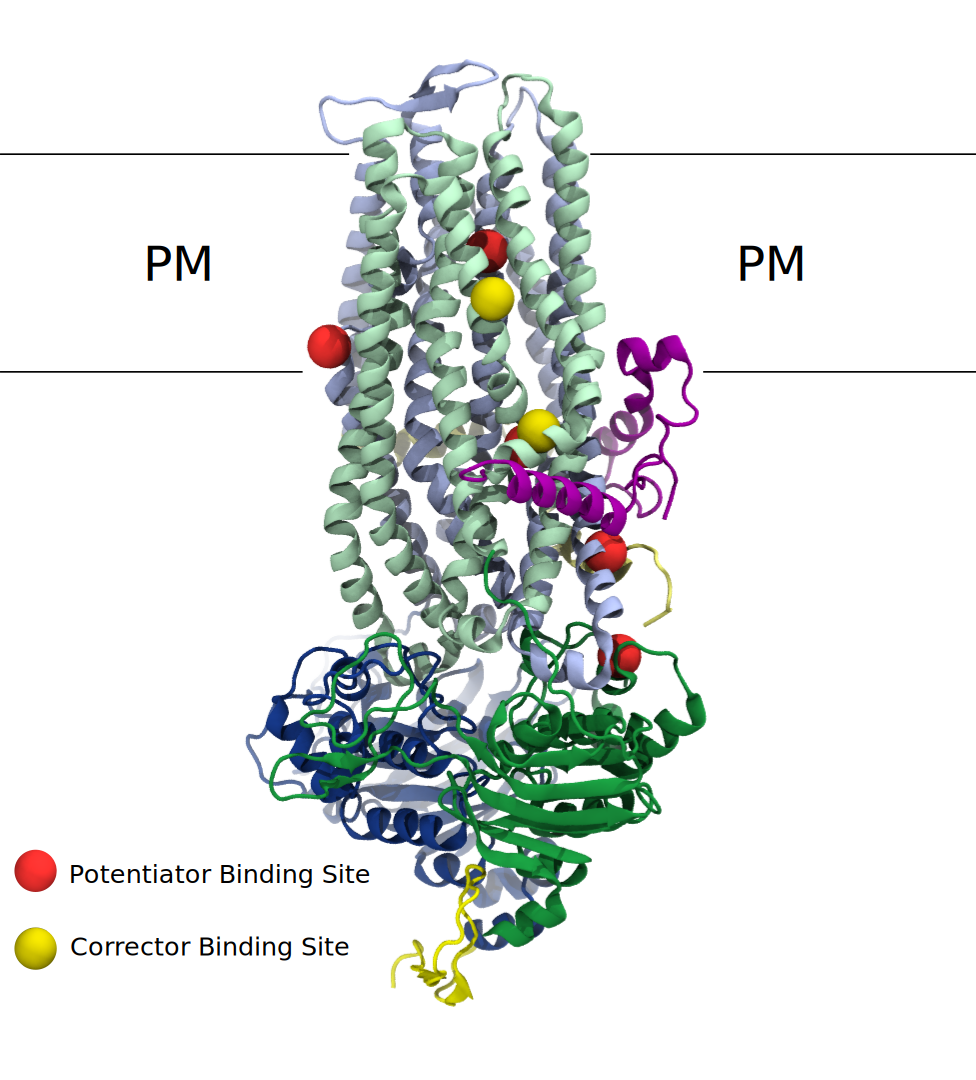
\includegraphics[width=0.6\textwidth]{figures/many_drug_sites.pdf}
\end{center}
\begingroup
\captionsetup{singlelinecheck = false, justification=raggedright}
\captionof{figure}[CFTR Has Many Proposed Drug Binding Sites]{\textbf{CFTR Has Many Proposed Drug Binding Sites} {There are many proposed sites in the literature where potentiators and correctors are proposed to dock to CFTR. All of the sites visualised here have been characterised through mutagenesis experiments or direct structural visualisation \cite{yeh2019, laselva2021a, liu2019, baatallah2021}. However, it is currently unclear which binding sites deliver the most clinical benefit. This gap in the literature could be filled by computational alchemical free energy calculations \cite{jorgensen2008,chipot2007}. }}
\label{many_drug_bound_CFTR}
\endgroup


Additionally, the model in chapter \ref{chap:perspective} should make it clear to the reader that the action of modulators is highly dependent on the underlying basic function of CFTR. These small molecule drugs \textit{select} for a physiologically present conformation, so we would wish to design molecules which select for conformations which deliver the most clinic benefit. This is non-trivial. A combination of careful molecular experiments, such as those of from the laboratories of Tzyh-Chang Hwang,  Christine E. Bear, L\'aszl\'o Csan\'ady and Paul Linsdell \cite{linsdell2018, csanady2019, laselva2022, zhang2017b}, and molecular simulations can help to understand which conformation the drugs are selecting for \cite{laselva2021a}.

Current generation modulators were identified using high throughput screening of different small molecules \cite{vangoor2009}. With the more powerful computational engines and artificial intelligences available today, alongside new biochemical and structural data, the next generation of modulators could be more targeted---perhaps even mutation specific.

%Specifically, there are now several proposed binding sites for many compounds on the CFTR protein. Some of these are better characterised than others but it is hotly debated which ones are important for the modulation of the protein (Figure \ref{many_drug_bound_CFTR}). A careful, systematic approach to calculations of the binding free energy of different drugs in each of these binding sites would be a great help to both a basic understanding of the protein, as well as drug discovery efforts. 

%The final element in this program is to understand, mechanistically, how small molecule drugs are compensating for the modified landscape exhibted by mutations. There are several unanswered questions surrounding how modulators restore CFTR function, but these are being studied intensly \cite{}. We propose that in silico characterisation, in parralel with these in vitro effors twill aid in efforts of both theratyping and drug discovery. As was observed in \ref{chap:cftr} the close integration of simulation studies ameliorates some of the challenges inherent to a computational appraoch. Therefore, we propose that future in silico efforts to elucidate the drug binding pockets of CFTR remain tightly integrated with in vitro experiments, until ocmputational methods are more mature. However, for already proposed drug binding pockets such as those proposed in \cite{}, it is likely that alchemical free energy calculations could provide significant mechanistic insight into he function of these CFTR modulators. These studies should be a priority for molecular studies of CFTR as they will have significant implications for drug discovery efforts and \textit{in vitro} investigations of these mechanisms can be challenging due to the hydrophobic nature of these drugs \cite{csanady2019}. 

%The most recent structure of human CFTR in a phosphorylated environment has some interesting features which have lead to some controversies in the literature. After spending significant time researching them I have conducted an extensive literature review in order to learn more about of these concerns. The released structure of activated, human CFTR has two features that have caused some in the CF field to suggest issues with this structure. Firstly, this structure is not sufficiently open to conduct chloride ions. Chloride ions have a diameter of 1.7$\angs$ while the structure has a constriction of 1.1$\angs$\cite{zhang2018}. So, there must be some level of conformational changes, even if chloride were to move through the channel completely dehydrated. This becomes even more of an issue when considers the experimental evidence where much larger anionic species such as bicarbonate and glutathione were shown to permeate through the channel \cite{kogan2003}. This suggests that there is a much larger conformation which has not been observed experimentally or in simulations. This was the motivation for chapter \ref{chap:opening} of this thesis. Some studies have been performed in order to study the possible permeation paths of chloride but they were usually not carried out on hCFTR or have not addressed the pressing question of how larger ions might permeate the channel \cite{farkas2020, zeng2021}. Bicarbonate in particular is of great physiological importance as there is a high correlation between the channel's ability to permeate bicarbonate and the pancreatic sufficiency of a patient carrying the mutation \cite{}. In light of this, structural knowledge of a fully open conformation of CFTR is critical to a personalised approach to the treatment of CFTR.
%The second and harder to resolve controversy concern the role of TM8. This transmembrane helix has an unusual bend in the middle of the plasma membrane. This is not something seen before in ABC transporters of this type. So it has led to some open questions as to how this bend might contribute to the function of the channel \textit{or} how it might be an artifact of the imaging process. For the former case, the structural biologists in the Chen lab proposed a mechanism whereby the upper hinge of TM8 swings 55$^o$ during the transition to the open state. This mechanism would give justification of the pathogenesis of certain mutaions such as L927P. 

%The arguments for the bend in the helix appear to be unphysical. In cryoEM structures, we can observe that the bent conformation is stabilised by salt bridges R347-D924 and E873-R933. The former bond has been well studied experimentally and was expected in the 3d structure. Additionally, all hydrogen bonds along the in the bent helix are . Been observed to be stable in MD \cite{corradi2018} .  is energetically stable.

%A study assessing the accuracy of Alphafold's predictions of transmembrane protein structures found an intersting result. When alphafold made predictions that involved the use of templates it predicts the unwound conformation of TM8. On the other hand, when templates are removed from alphafolds predictions it predicts a straight TM8 conformation, very similar to that found in chCFTR. The authors of this study suggested the reason for the discrepancy was due to the use of detergents in the deteremination of the structure of hCFTR. However, careful reading of cryo-EM literature reveals no examples where the use of detergents has resulted in such drastic conformational changes. One of the few examples where both detergents and native-like nanodisks were used to determine the structure of a protein are the determinations of the structure of TRPV1. These studies revealed no difference to the backbone helices but did suggest important information about the importance of different interactions with lipids \cite{gao2016}. A lot of work has been performed in order to create detergents which reflect a native lipid environment and these are the species that were used in the determination of the human CFTR structure (albeit at a higher than optimal concentration) \cite{gao2016, zhang2018, kampjut2021}. 

%The authors of the chCFTR paper suggested that the different expression systems used in the two studies could be the reason for the discrepancy between the two systems, due it their different post translational processing apparatus. Although both groups used mammalian cell lines the chCFTR paper used hamster? cells \cite{aleksandrov2015} and the Chen lab used HEK293S cells. The chicken structure also underwent significant mutations in order to be locked open and imaged. The regulatory insertion was deleted in order to aid in the purification of the protein. 

%The molecular and cellular basis behind this heterogeneous response is thus of critical importance to CF care and is only recently being addressed in the literature \cite{}. The metabolism of these drugs is under study, in order to understand this patient specific response \cite{hanafin2021}. A complimetnary therapeutic which addresses the root cause of this issue would greatly increase patient outcomes. Sadly, such studies are far outside the reach of computaitonal biology at the moment and so we encourage careful clinical research to test for genetic or environmental factors which cause patients to not respond to modulators. In the mean-time, a pre-clinical approach such as the one undertaken by the collaborators of this thesis can rationally expand the number of patients who will receive these therapies.

%Trikafta triple therapy is changing the face of mutation specific therapy. For example, N1303K, a common mutation, which does not respond to potentiators or correctors by thesemselves, or even together \cite{} does respond to triple therapy. This is a similar situation for rarer mutations like R560S, which is rarer and so has not yet been tested for efficacy with the triple therapy \cite{awatade2019}. In summary, given the results from this thesis we expect that the majority of missense mutations will respond to a triple therapy. Patients carrying these genotypes who do not respond to triple therapy likely have factors \textit{beyond} the physical action of the modulators on CFTR which are . It is possible that exceptions do exist and the physical model proposed in this chapter will help us form a physical basis for which ones can be excluded. To account for these factors a patient specific pre-clinical approach will help us predict which patients respond to these medications and eventually pin down which cellular factors are preventing the rescue of chloride transport in these patients. The maturation of this technology will bring considerable therapeutic benefit to CF patients and eventually those suffering from other diseases too.

%These drugs are clinically efficacious \cite{VanGoor2014} on several mutants with some curious exceptions like N1303K. I suggest the following mechanism for their action. I suspect a similar analogy exists for the action of the correctors. WT-CFTR exhibits a natural landscape with kinetic barriers in the transition between the closed and open states. A gating class mutation to CFTR will introduce a kinetic barrier in the pathway of this conformational transition. What these drugs do is reduce a barrier in the existing conformational landscape of CFTR. This compensates for the barriers introduced by the mutation. j
